\documentclass[a4paper,10pt]{article}
\usepackage[utf8]{inputenc}

\usepackage{graphicx}
\usepackage{subfigure}
\usepackage{caption}
% \usepackage{float}
% \usepackage{ucs} 
% \usepackage{subcaption}
\usepackage{pgfplots}
\def\func1(#1,#2){exp(-(#1-#2)^2/(0.01))}
\usepackage{tikz}

\usetikzlibrary{shapes,arrows}
\usetikzlibrary{arrows,calc}

\tikzset{
    block/.style = {draw, rectangle, 
        minimum height=1cm, 
        minimum width=1.2cm},
    input/.style = {coordinate,node distance=1cm},
    output/.style = {coordinate,node distance=2cm},
    arrow/.style={draw, -latex,node distance=1.5cm},
    pinstyle/.style = {pin edge={latex-, black,node distance=1.5cm}},
    sum/.style = {draw, circle, node distance=1cm}
}

\usepackage{psfrag}
\usepackage{verbatim}
\usepackage{amsmath}
\usepackage{amsfonts} 
\usepackage{pifont}
\newcommand{\cmark}{\ding{51}}%
\newcommand{\xmark}{\ding{55}}%
\usepackage{amssymb} 
\usepackage{amsthm}
\usepackage{tikz}
 \usetikzlibrary{calc}
\usepackage{array}
\usepackage{verbatim}
\usepackage{listings}
\usepackage{stfloats}
    \DeclareMathOperator{\atan}{atan}
    \DeclareMathOperator{\acos}{acos}
    \DeclareMathOperator{\asin}{asin}
\usepackage{algorithm} 
\usepackage{algorithmic} 
\usepackage{url} 
  \usepackage{enumerate}
\usepackage{multirow}
\usepackage{wasysym}
\usepackage{cancel}


% Comando para evitar warning por tamaños de fonte. Se se empregan as fontes lmodern non se precisa e debe ser comentado.
\let\Tiny = \tiny

% CREACIÓN DUN COMANDO QUE INTRODUCE UNHA DIAPOSITIVA CUN ÍNDICE NO QUE APARECEN VELADAS TÓDALAS SECCIÓNS MENOS A ACTUAL. ÚTIL PARA INTRODUCIR OS TÍPICOS ÍNDICES INTERMEDIOS.
\renewcommand{\figurename}{Fig.}

\newcommand{\field}[1]{\mathbb{#1}}

\newcommand{\Hb}{\mathbf{H}}
\newcommand{\Sb}{\Sigma}
\newcommand{\Sm}{\mathbf{S}}
\newcommand{\U}{\mathbf{U}}
\newcommand{\F}{\mathbf{F}}
\newcommand{\V}{\mathbf{V}}
\newcommand{\A}{\mathbf{A}}
\newcommand{\B}{\mathbf{B}}
\newcommand{\Cb}{\mathbf{C}}
\newcommand{\D}{\mathbf{D}}
% \newcommand{\E}{\mathbf{E}}
\newcommand{\T}{\mathbf{T}}
\newcommand{\I}{\mathbf{I}}
\newcommand{\Y}{\mathbf{Y}}
\newcommand{\M}{\mathbf{M}}
\newcommand{\N}{\mathbf{N}}
\newcommand{\W}{\mathbf{W}}
\newcommand{\Z}{\mathbf{Z}}
\newcommand{\R}{\mathbf{R}}
\newcommand{\K}{\mathbf{K}}
\newcommand{\X}{\mathbf{X}}
\newcommand{\Pb}{\mathbf{P}}
\newcommand{\Lb}{\mathbf{L}}
\newcommand{\Phib}{\mathbf{\boldsymbol{\Phi}}}
\newcommand{\Upsb}{\mathbf{\boldsymbol{\Upsilon}}}
\newcommand{\Q}{\mathbf{Q}}
% \newcommand{\D}{\mathbf{D}}
\newcommand{\one}{\mathbf{1}}
\newcommand{\zero}{\mathbf{0}}
\newcommand{\Rm}{\mathbf{R^{-1}}}
\newcommand{\LL}{\mathbf{\boldsymbol{\Lambda}}}
\newcommand{\J}{\mathbf{J}}

\newcommand{\cc}{\mathbf{c}}
\newcommand{\h}{\mathbf{h}}
\newcommand{\x}{\mathbf{x}}
\newcommand{\f}{\mathbf{f}}
\newcommand{\s}{\mathbf{s}}
\newcommand{\q}{\mathbf{q}}
\newcommand{\vv}{\mathbf{v}}
\newcommand{\uu}{\mathbf{u}}
\newcommand{\y}{\mathbf{y}}
\newcommand{\bb}{\mathbf{b}}
\newcommand{\n}{\mathbf{n}}
\newcommand{\w}{\mathbf{w}}
\newcommand{\e}{\mathbf{e}}
\newcommand{\uv}{\mathbf{u}}
\newcommand{\al}{\mathbf{\boldsymbol{\alpha}}}
\newcommand{\vmu}{\mathbf{\boldsymbol{\mu}}}
\newcommand{\vlambda}{\mathbf{\boldsymbol{\lambda}}}
\newcommand{\g}{\mathbf{g}}
\newcommand{\rr}{\mathbf{r}}
\newcommand{\z}{\mathbf{z}}
\newcommand{\ab}{\mathbf{a}}
\newcommand{\pp}{\mathbf{p}}

\newcommand{\pd}[2]{\frac{\partial #1}{\partial #2}}
\newcommand{\pw}[1]{\frac{\partial #1}{\partial \w}}


\newcommand{\rank}{\textnormal{rank}}
\newcommand{\trace}{\textnormal{trace}}
\newcommand{\exptr}{\textnormal{exptr}}
\newcommand{\tr}{\textnormal{tr}}
\newcommand{\vstack}{\textnormal{vec}}
\newcommand{\diag}{\textnormal{diag}}
%  |x>
\newcommand{\ket}[1]{\left\vert#1\right\rangle}
%  <x|
\newcommand{\bra}[1]{\left\langle#1\right\vert}
%  <x|y>
\newcommand{\braket}[2]{\left< #1 \vphantom{#2}\,
                        \right\vert\left.\!\vphantom{#1} #2 \right>}
%  <x|a|y>
\newcommand{\sandwich}[3]{\left< #1 \vphantom{#2 #3} \right|
                          #2 \min\left(\vphantom{#1 #2} #3 \right>}
%  d/dt
\newcommand{\ddt}{\frac{d}{dt}}
%  D/Dx
\newcommand{\pdd}[1]{\frac{\partial}{\partial#1}}
%  |x|
\newcommand{\abs}[1]{\left\vert#1\right\vert}
%  k_{x}
\newcommand{\kv}[1]{\mathbf{k}_{#1}}
%  \textnormal{E}_{domain of integration}{variable}
\newcommand{\Ex}[2]{{\textnormal{E}_{#1}\left[#2\right]}}
\newcommand{\CEx}[3]{{\textnormal{E}_{#1}\left[#2|#3\right]}}
\newcommand{\CInf}[3]{{\textnormal{I}\left(#1;#2|#3\right)}}
\newcommand{\Inf}[2]{{\textnormal{I}\left(#1;#2\right)}}
\newcommand{\CEnt}[2]{{\textnormal{H}\left(#1|#2\right)}}
\newcommand{\Ent}[1]{{\textnormal{H}\left(#1\right)}}
\newcommand{\dCEnt}[2]{{\textnormal{h}\left(#1|#2\right)}}
\newcommand{\dEnt}[1]{{\textnormal{h}\left(#1\right)}}

\newcommand\Tau{\mathcal{T}}
% \newtheorem{definition}{Definition}

\newcommand{\tikzmark}[1]{\tikz[overlay,remember picture] \UE (#1) {};}
\newcommand{\DrawBox}[4][]{%
    \tikz[overlay,remember picture]{%
        \coordinate (TopLeft)     at ($(#2)+(-0.4em,1.6em)$);
        \coordinate (BottomRight) at ($(#3)+(0.4em,-1.0em)$);
        %
        \path (TopLeft); \pgfgetlastxy{\XCoord}{\IgnoreCoord};
        \path (BottomRight); \pgfgetlastxy{\IgnoreCoord}{\YCoord};
        \coordinate (LabelPoint) at ($(\XCoord,\YCoord)!0.5!(BottomRight)$);
        %
        \draw [red,#1] (TopLeft) rectangle (BottomRight);
        \UE [below, #1, fill=none, fill opacity=1] at (LabelPoint) {#4};
    }
}
%   \usepackage[pdftex]{graphicx}
  \usepackage{epstopdf}
   \graphicspath{{./img/}}
  % and their extensions so you won't have to specify these with
  % every instance of \includegraphics
   \DeclareGraphicsExtensions{.eps,.png,.jpg}
   
   
% \newtheorem{definition}{Definition}
% \newtheorem{lemma}{Lemma}
% \newtheorem{theorem}{Theorem}
\newtheorem{remark}{Remark}
\newtheorem{proposition}{Proposition}
% \newtheorem{corollary}{Corollary}
% \newtheorem{example}{Example}
\newtheorem{homework}{Homework}
   
   \definecolor{VCobalt}{HTML}{005682} % a mate dark blue
   \definecolor{TZTeal}{HTML}{008080} % a mate dark teal
   \definecolor{KYJade}{HTML}{008151} % a mate dark green
   \definecolor{ARust}{HTML}{a10000} % a mate dark red
   \definecolor{blueH3}{rgb}{0,.5,1} % a ligher blue
   \definecolor{blueH2}{rgb}{0,0.25,0.75} % a medium blue
   \definecolor{blueH1}{rgb}{0,0,0.5} % a darker blue
   \definecolor{GPSCCommonBlue}{HTML}{005f86} % Nuria's reference

%opening
\title{Extra Exercises for SACOM 2020}
\author{Felipe Gomez Cuba}

\begin{document}

\section{Book}

You can check the exercises in Chapters 6 and 10 of the freely available book ``David Tse, Pramod Viswanath, Fundamentals of Wireless Communication, Cambridge University Press, 2005''. Note that some of these exercises require very advanced deductions that go beyond the scope of our course. Also bear in mind that some of these exercises are focused on CDMA systems that are not as relevant nowadays.

\section{Example Exam Problems}
\subsection{Equal Capacity MAC (Exam 2015)}

Consider an AWGN SISO MAC channel with $U$ users. Prove that the capacity of all users is the same if the received power is of the form $P_n=\alpha^n\beta, n\in\{1\dots U\}$. The noise power at the receiver is denoted by $\sigma^2$ and the users are decoded in order $1,2,\dots U$. Obtain $\alpha$ and $\beta$ as a function of the SNR of user $U$ denoted by $snr_U=\frac{P_U}{\sigma^2}$

\subsection{BC Power Allocation}

Consider a AWGN SISO BC with $2$ users with channels ordered $|h_1|<|h_2|$. 
\begin{enumerate}
 \item Show that the power allocation $P_1+P_2=P$ that maximizes the sum rate if we employ the capacity-achieving SIC receiver technique is $P=P_2$. (Hint: recall that $\log(1+A/B)=\log(B+A)-\log(B)$)
 \item Since the max sum rate criterion makes the BC channel leave some users without any service, we must consider other goals for power allocation. Find $P_1$ and $P_2$ such that both users achieve equal rates.
 \item Consider now a TDMA orthogonal scheme with time division $\frac{1}{2}$ in the same BC channel. Now we interpret $P_1$ and $P_2$ as the ``instanatenous'' power each user user transmits in its interval. Write the rate expressions and find $P_1$ and $P_2$ for equal rate.
\end{enumerate}

\section{Advanced Problems}
\subsection{QR Factorization DPC BC}

Consider a $K$ user BC with $N_t>K$ transmit antennas at the transmitter and a single antenna in each receiver. The equivalent channel is written as
$$\y=\Hb^H\x+\z$$

Instead of the conventional DPC scheme to achieve capacity, we consider a scheme based on the QR factorization of $\Hb=\Q\R$ where $\R$ is upper triangular an $\Q$ is an unitary matrix satisfying $\Q^H\Q=\I$. The transmitted signal is $$\x=\Q\left(\begin{array}{c}x_1\\x_2\\\vdots\\x_k\\0\\\vdots\\0_{N_t-K}\end{array}\right).$$

\begin{enumerate}
 \item Calculate the SINR of each user $k$ as a function of $r_{k,k'}$ if the transmitter encodes $x_{k}$ using DPC with known $x_{1}\dots x_{k-1}$.
\end{enumerate}

\subsection{MAC Power Control}

In practice, many systems implement \textit{power control}. For example in cellular systems of generations 3G to 5G, due to hardware implementation requirements all received signals at the BS must have the same \textit{received} power. Consider a 2 user SIMO MAC channel $N$ receive antennas at the receiver
$$\y=\h_1 x_1+\h_2 x_2+\z,$$
, representing two mobile phones User Equipment (UE) transmitting to the same Base Station (BS). The transmitted power of each transmitter is $\Ex{}{|x_i|^2}=P_i = P_{\max}*10^{-\frac{\beta_i}{10}}$ where $P_{\max}$ is the maximum transmit power of the mobile phones and the parameter $\beta_i$ [in dB] is called the ``power control back-off'' of user $i$.

\begin{enumerate}
 \item Calculate $\beta_1$ and $\beta_2$ such that the received powers of both signals are equal.
 \item Assuming a simple Matched Filter linear combiner is employed at the receiver, calculate the SINRs and ``achievable rates'' of both users. 
\end{enumerate}


% \subsection{Cooperative Multi-Point}
% Consider a CoMP mobile cellular system as in Fig. \ref{fig:comp} where a cloud server performs signal processing for two base stations at once. There are two mobile towers at different locations acting as two SISO receivers and there are 2 users acting as transmitters, one near each tower. Each receiver $i$ sees the channel 
%     $$y_i=h_{1,i}x_1+h_{2,i}x_2+z_i$$ 
%     
%     \begin{figure}[h]
%     \centering
%         \begin{tikzpicture}[scale=.5]
%             \draw [->] (.75,2.25) -- (8.25,1.25);
%             \draw [->] (.75,-2.25) -- (8.25,-1.25);
%             \draw [->] (.75,2.25) -- (8.25,-.75);
%             \draw [->] (.75,-2.25) -- (8.25,.75);
%             \node at (0,2.5) {$x_1$};
%             \node at (0,-2.5) {$x_2$};
%             \draw (9,1) circle (.75);
%             \draw (0,2.5) circle (.75);
%             \draw (9,-1) circle (.75);
%             \draw (0,-2.5) circle (.75);
%             \node[block] (server) at (12,0) {Server};
%             \draw[->] (9.5,.5) -- (server);
%             \draw[->] (9.5,-.5) -- (server);
%             \node at (9,1) {$y_1$};
%             \node at (9,-1) {$y_2$};
%     %                 \draw (6,0) ellipse (1 and 2.5) dashed;
%             \node[anchor=south] at (5.5,1.25) {$h_{1,1}$};
%             \node[anchor=south] at (2,0) {$h_{1,2}$};
%             \node[anchor=north] at (2,0) {$h_{2,1}$};
%             \node[anchor=north] at (5.5,-1.25) {$h_{2,2}$};
%         \end{tikzpicture}
%         \caption{A CoMP $2$-antenna SIMO MAC channel}
%         \label{fig:comp}
%      \end{figure}
%      \begin{itemize}
%       \item In the \textbf{standalone} mode of operation receiver $1$ decodes $x_1$ treating $h_{2,1}x_2$ as noise and assuming $h_{2,1}x_2\sim\mathcal{CN}(0,|h_{2,1}|^2P_2)$, and vice-versa.
%       \item In \textbf{CoMP} mode both receivers send $y_1$ and $y_2$ to a cloud server. The server creates a joint vector $\y=(y_2,y_2)^T$ and decodes $x_1$ and $x_2$ jointly from $\y$ using SIC. 
%      \end{itemize}
%      
%      \begin{enumerate}
%       \item Write the MIMO DEC for the CoMP case using the notation $\x=(x_1,x_2)^T$.
%       \item Write the SINR for both cases
%       \item Write a sum-rate expression in both cases
%       \item Show that $R_1^{standalone}+R_2^{standalone}\leq R_1^{CoMP}+R_2^{CoMP}$ (Hint: use the chain rule)
%      \end{enumerate}
% 
% 

\subsection{MMSE receiver implementation}

 Using the Matrix Inversion Lemma we have $$\W_{MMSE}=\left(\Hb^H\Hb+\sigma^2\I\right)^{-1}\Hb^H=\Hb^H\left(\Hb\Hb^H+\sigma^2\I\right)^{-1}.$$
Thus for single antenna transmitters and $N$-antenna receiver, the MMSE filter can be regarded as a bench of single-user filters $r_i=\w^H_i\y$ where the filter of user $i$ is
$$\w_i^H=\h_i^H\left(\Hb\Hb^H+\sigma^2\I\right)^{-1}$$
Write the explicit expression for the SINR of user $i$ ($\gamma_i$) in a MMSE MAC receiver with $U$ users as a function of $\h_i$, $\h_{j\neq i}$, $\Hb$, $P_i$, $P_{j\neq i}$, and $\sigma_z^2$.

\subsection{Imperfect CSI}

In practice the receiver needs to estimate the channel $\h$ before using this value in the receiver algorithms. To model imperfect knowledge of $\h$, let us assume that the receiver only has access to a noisy observation of the channel written as $\hat{\h}=\h+\e$, where $\e\sim\mathcal{CN}(0,\sigma_e^2\I)$. This is true in multi-user systems as well but to make this exercise shorter we will focus on the single-user case. Thus, a single-user channel can be written as
     $$\y=\hat{\h}x-\e x+\z$$
where $\Ex{}{|x|^2}=P$,  $\Ex{}{\z\z^H}=\sigma_z^2\I$. $\e$ is also independent of $x$.
     

\begin{enumerate}
 \item Design a MMSE receive filter $\w^H$ as the solution to $\min\Ex{}{| \w^H\y - x |^2}$. The result should be an expression depending on the \textbf{known} parameters $\hat{\h}$, $\sigma_e^2$, $\sigma_z^2$ and $P$.
\end{enumerate}
 
\subsection{Analog beamforming}

Sometimes due to hardware cost limitations transmitters and receivers with many omnidirectional antennas are converted into an ``equivalent single antenna'' radio, using analog circuits to implement a fixed beamforming vector. Consider a 2 user MAC channel with a large number of antennas in each device. Each transmitter $i$ projects the scalar signal $s_i[n]$ to its multiple antennas using a \textit{precoding vector} $\vv_i$, creating the transmitted signal 
$$\x_i[n]=\vv_i s_i[n].$$
The receiver has two ``analog beamforming'' circuits as well, denoted $\w_1^H$ and $\w_2^H$, and the received signal at their outputs is
$$\y=\left(\begin{array}{c}\w_1^H\\\w_2^H\end{array}\right)\left(\Hb_1\x_1+\Hb_2\x_2\right)+\z$$
The practical use of the analog beamforming sytem is to simplify the hardware. Each transmitter behaves as if it had a ``single directive antenna'' pointed at the receiver, and the receiver behaves as if it had ``two directive antennas'' pointed at the transmitter. This means that we can model the digital channel as a $2\times2$ MIMO equivalent expression as follows
$$\y=\Hb_{eq}\left(\begin{array}{c}s_1\\s_2\end{array}\right)+\z$$
\begin{enumerate}
 \item Write the expresion for the equivalent channel matrix $\Hb_{eq}$ as a function of $\vv_1$,  $\vv_2$, $\w_1^H$, $\w_2^H$ and $\Hb$.
 \item Write the SINRs if a MMSE filter of size $2\times 2$ is enployed at the receiver.
\end{enumerate}



\subsection{Wideband Multi-user systems}

Recall that in the single-user channel the rate was power-limited according to the asymptotic result $\lim_{B\to\infty}B\log(1+\frac{P|h|^2}{N_oB})=\frac{P|h|^2}{N_o}\log_2e$. Show that FDMA schemes are asymptotically optimal for a SISO MAC channel in the limit as the bandwidth goes to infinity.

\subsection{Multi-user Diversity Gain}

Consider a $K$ user FDMA SISO BC fast fading channel employing a maximum-throughput scheduler. The channel coefficients are Rayleigh independent identically distributed for each user $h_k\sim \mathcal{CN}(0,\sigma_h^2)$. Find the \textbf{multi-user diversity gain} defined as $G=\frac{\Ex{}{\max |h_k|^2}}{\sigma_h^2}$. Use the following identities:
\begin{itemize}
 \item For exponential distributions $f(x)=\lambda e^{-\lambda x}$, $F(x)=1-e^{-\lambda x}$
 \item If $X_1,X_2$ are independent then
 $$P(\max(X_1,X_2)\leq x)=P(X_1\leq x)P(X_2\leq x)$$
 \item If $X$ is a random variable with positive support then
 $$\Ex{}{X}=\int_{e=0}^{\infty} 1-F_{X}(x)dx$$
 \item Binomial Theorem: $(1+x)^K=\sum_{n=0}^{K}{K \choose n}x^{n}$
\end{itemize}
(Note: leave the result as a series sum with a combinatorial expression that depends on $K$ and $n$, you don't have to solve the sum)

\subsection{Path Diversity}

Consider a Degraded Relay Channel with $K$ Relays as in Fig. \ref{fig:mpdiv}. We assume \textbf{only one} relay can be active at any time. The network control entity must select the best relay to repeat the signal received from the transmitter. Assumie static DF with a time division $1/2$ is employed and the signal from the source $\x$ is not received by the final destination. All transmitters have the same power $P$ and all receivers experience the same noise variance $\sigma^2$.

\begin{itemize}
 \item Write the rate that could be achieved by each relaying path $R_k$ as a function of the channels $\Hb_{XR,k}$ and $\Hb_{RY,k}$.
 \item Assuming that all the devices have a single antenna, if we wish to choose the relay that achieves the best rate $R_k$, write the achieved rate as a function of $|h_{XR,k}|^2$ and $|h_{RY,k}|^2$.
\end{itemize}


  
    \begin{figure}[h]
    \centering
        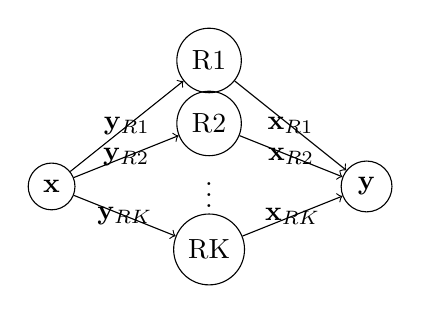
\begin{tikzpicture}[scale=.4]
            \node[draw,circle] (tx) at (0,0) {$\x$};
            \node[draw,circle] (rx1) at (5,4) {R1};
            \node[draw,circle] (rx2) at (5,2) {R2};
            \node (rx3) at (5,0) {$\vdots$};
            \node[draw,circle] (rx4) at (5,-2) {RK};
            \node[draw,circle] (rx) at (10,0) {$\y$};
            \draw[->] (tx) -- node {$\y_{R1}$} (rx1);
            \draw[->] (tx) -- node {$\y_{R2}$} (rx2);
            \draw[->] (tx) -- node {$\y_{RK}$} (rx4);
            \draw[->] (rx1) -- node {$\x_{R1}$} (rx);
            \draw[->] (rx2) -- node {$\x_{R2}$} (rx);
            \draw[->] (rx4) -- node {$\x_{RK}$} (rx);
        \end{tikzpicture}
        \caption{Oportunistic Relaying with multiple relays}
        \label{fig:mpdiv}
     \end{figure}

\end{document}
